\documentclass{article}

\usepackage[bookmarksnumbered, colorlinks, plainpages]{hyperref}
\usepackage{fancyhdr}
\usepackage{extramarks}
\usepackage{amsmath}
\usepackage{amsthm}
\usepackage{amsfonts}
\usepackage{tikz}
\usepackage[plain]{algorithm}
\usepackage{algpseudocode}
\usepackage{graphicx}
\usepackage{tabularx}

\graphicspath{ {./img/} }
\usetikzlibrary{automata, positioning}

%
% Basic Document Settings
%

\topmargin=-0.45in
\evensidemargin=0in
\oddsidemargin=0in
\textwidth=6.5in
\textheight=9.0in
\headsep=0.25in

\linespread{1.1}

\pagestyle{fancy}
\lhead{\hmwkAuthorName}
\chead{\hmwkClass\ (\hmwkClassInstructor\ \hmwkClassTime): \hmwkTitle}
\rhead{\firstxmark}
\lfoot{\lastxmark}
\cfoot{\thepage}

\renewcommand\headrulewidth{0.4pt}
\renewcommand\footrulewidth{0.4pt}

\setlength\parindent{0pt}

%
% Create Problem Sections
%

\newcommand{\enterProblemHeader}[1]{
    \nobreak\extramarks{}{Problem \arabic{#1} continued on next page\ldots}\nobreak{}
    \nobreak\extramarks{Problem \arabic{#1} (continued)}{Problem \arabic{#1}
    continued on next page\ldots}\nobreak{}
}

\newcommand{\exitProblemHeader}[1]{
    \nobreak\extramarks{Problem \arabic{#1} (continued)}{Problem \arabic{#1}
    continued on next page\ldots}\nobreak{}
    \stepcounter{#1}
    \nobreak\extramarks{Problem \arabic{#1}}{}\nobreak{}
}

\setcounter{secnumdepth}{0}
\newcounter{partCounter}
\newcounter{homeworkProblemCounter}
\setcounter{homeworkProblemCounter}{1}
\nobreak\extramarks{Problem \arabic{homeworkProblemCounter}}{}\nobreak{}

%
% Homework Problem Environment
%

\newenvironment{homeworkProblem}[1]{
    \section{Problem \arabic{homeworkProblemCounter}{#1}}
    \setcounter{partCounter}{1}
    \enterProblemHeader{homeworkProblemCounter}
}{
    \exitProblemHeader{homeworkProblemCounter}
}

%
% Homework Details
%   - Title
%   - Due date
%   - Class
%   - Section/Time
%   - Instructor
%   - Author
%

\newcommand{\hmwkTitle}{Homework\ 7}
\newcommand{\hmwkDueDate}{April 12, 2024}
\newcommand{\hmwkClass}{CS 362}
\newcommand{\hmwkClassTime}{11:00am}
\newcommand{\hmwkClassInstructor}{Professor Troy}
\newcommand{\hmwkAuthorName}{\textbf{Ryan Magdaleno}}
\newcommand{\hwline}{\begin{center}\line(1,0){358px}\end{center}}

%
% Title Page
%

\title{
    \vspace{2in}
    \textmd{\textbf{\hmwkClass:\ \hmwkTitle}}\\
    \normalsize\vspace{0.1in}\small{Due\ on\ \hmwkDueDate\ at 11:59pm}\\
    \vspace{0.1in}\large{\textit{\hmwkClassInstructor\ \hmwkClassTime}}
    \vspace{3in}
}

\author{\hmwkAuthorName\\\href{mailto:rmagd2@uic.edu}{rmagd2@uic.edu}}
\date{}

\renewcommand{\part}[1]{\textbf{\large Part \Alph{partCounter}}
\stepcounter{partCounter}\\}
%
% Various Helper Commands
%

% Useful for algorithms
\newcommand{\alg}[1]{\textsc{\bfseries \footnotesize #1}}

% For derivatives
\newcommand{\deriv}[1]{\frac{\mathrm{d}}{\mathrm{d}x} (#1)}

% For partial derivatives
\newcommand{\pderiv}[2]{\frac{\partial}{\partial #1} (#2)}

% Integral ds
\newcommand{\dx}{\mathrm{d}x}
\newcommand{\D}[1]{\mathrm{d}#1}

% Image insertion
\newcommand{\img}[2]{\begin{center}\includegraphics[scale=#1]{#2}\end{center}}

% Alias for the Solution section header
\newcommand{\solution}{\textbf{\large Solution}\\}

% Probability commands: Expectation, Variance, Covariance, Bias
\newcommand{\E}{\mathrm{E}}
\newcommand{\Var}{\mathrm{Var}}
\newcommand{\Cov}{\mathrm{Cov}}
\newcommand{\Bias}{\mathrm{Bias}}

\begin{document}

\maketitle

\pagebreak

%%%%%%%%%%%%%%%%%%%%%%%%%%%%%%%%%%%%%%%%%%%%%%%%%%%%%%%%%%%%%%%%%%%%%%%%%%%%%%%%%%%%%%%%%

\begin{homeworkProblem}{}
    Consider the following Finite State Machine:\\
    Start State: A\\
    Inputs are listed before the slash on each transition.\\
    Outputs are listed after the slash on each transistion.
    \img{0.3}{1.png}
    \hwline\solution
    \begin{enumerate}
        \item\vspace{-5pt}
        Is the above FSM a Moore machine or a Mealy machine? \\
        Mealy Machine.
        \hwline
        \item\vspace{-5pt}
        What is output by the above FSM for:\\
        Input: 1 0 1 1 0 0 0 1 0 0 1 1 \\
        Output: 0 0 1 0 0 0 0 0 0 0 0 0
        \hwline
        \item\vspace{-5pt}
        Give the truth table for the above Finite State Machine. \\
        Encode the states using “one hot bit” encoding values of: $A\rightarrow$ 001, 
        $B\rightarrow$ 010, $C\rightarrow$ 100 \\
        \begin{tabularx}{0.9\textwidth} { 
            | >{\centering\arraybackslash}X 
            | >{\centering\arraybackslash}X 
            | >{\centering\arraybackslash}X 
            | >{\centering\arraybackslash}X 
            | >{\centering\arraybackslash}X 
            | >{\centering\arraybackslash}X 
            | >{\centering\arraybackslash}X 
            | >{\centering\arraybackslash}X | }
            \hline $p2$ & $p1$ & $p0$ & $b$ & $y$ & $n2$ & $n1$ & $n0$ \\
            \hline 0 & 0 & 1 & 0 & 0 & 0 & 0 & 1 \\
            \hline 0 & 0 & 1 & 1 & 0 & 0 & 1 & 0 \\
            \hline 0 & 1 & 0 & 0 & 0 & 1 & 0 & 0 \\
            \hline 0 & 1 & 0 & 1 & 0 & 0 & 1 & 0 \\
            \hline 1 & 0 & 0 & 0 & 0 & 0 & 0 & 1 \\
            \hline 1 & 0 & 0 & 1 & 1 & 0 & 1 & 0 \\
            \hline
        \end{tabularx}
        \hwline
        \pagebreak
        \item\vspace{-5pt}
        Write out the simplified expressions for the next state and output values. \\
        You can use K-maps or boolean algebra to determine simplified expressions. \\
        Show your work.
        \img{0.3}{1a.png}
        \img{0.2}{1b.png}
        \hwline
        \pagebreak
        \item\vspace{-5pt}
        Draw the circuit diagram for the Finite State Machine. \\
        Use the format as shown in class and in the zyBooks (and in following programs) 
        that contain a state register and a combination logic block.
        \img{0.2}{1c.png}
    \hwline
    \end{enumerate}
\end{homeworkProblem}
\pagebreak

%%%%%%%%%%%%%%%%%%%%%%%%%%%%%%%%%%%%%%%%%%%%%%%%%%%%%%%%%%%%%%%%%%%%%%%%%%%%%%%%%%%%%%%%%

\begin{homeworkProblem}{}
    Suppose we have a machine that takes in an infinite stream of bits, one bit at a time.
    On every input, the machine will output '0', unless the machine has seen the pattern 
    '10101' in the last four inputs where it will instead output '1'. \\
    Below is an example of this behavior. \\
    Input: 010101010010101011101010... \\
    Output: 000001010000001010000010...
    \hwline\solution
    \begin{enumerate}
        \item\vspace{-5pt}
        Design/Draw an FSM that exhibits the behavior described above.
        \begin{center}
            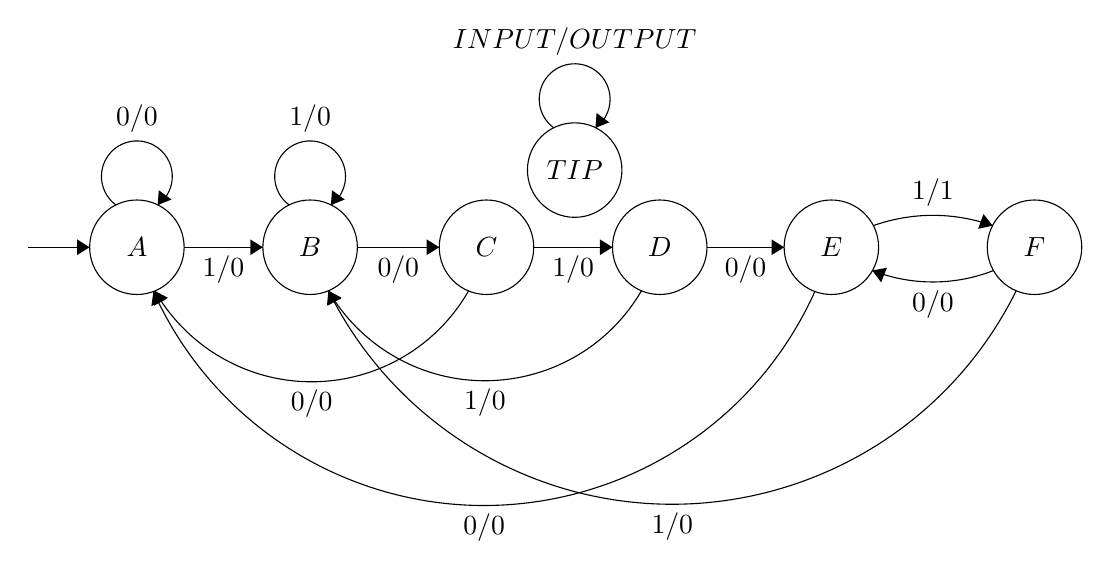
\begin{tikzpicture}[scale=0.2]
            \tikzstyle{every node}+=[inner sep=0pt]
            \draw [black] (41.9,-27.8) circle (3);
            \draw (41.9,-27.8) node {$TIP$};
            \draw [black] (14.1,-32.7) circle (3);
            \draw (14.1,-32.7) node {$A$};
            \draw [black] (25.1,-32.7) circle (3);
            \draw (25.1,-32.7) node {$B$};
            \draw [black] (36.3,-32.7) circle (3);
            \draw (36.3,-32.7) node {$C$};
            \draw [black] (47.3,-32.7) circle (3);
            \draw (47.3,-32.7) node {$D$};
            \draw [black] (58.2,-32.7) circle (3);
            \draw (58.2,-32.7) node {$E$};
            \draw [black] (71.1,-32.7) circle (3);
            \draw (71.1,-32.7) node {$F$};
            \draw [black] (40.577,-25.12) arc (234:-54:2.25);
            \draw (41.9,-20.55) node [above] {$INPUT/OUTPUT$};
            \fill [black] (43.22,-25.12) -- (44.1,-24.77) -- (43.29,-24.18);
            \draw [black] (7.2,-32.7) -- (11.1,-32.7);
            \fill [black] (11.1,-32.7) -- (10.3,-32.2) -- (10.3,-33.2);
            \draw [black] (17.1,-32.7) -- (22.1,-32.7);
            \fill [black] (22.1,-32.7) -- (21.3,-32.2) -- (21.3,-33.2);
            \draw (19.6,-33.2) node [below] {$1/0$};
            \draw [black] (28.1,-32.7) -- (33.3,-32.7);
            \fill [black] (33.3,-32.7) -- (32.5,-32.2) -- (32.5,-33.2);
            \draw (30.7,-33.2) node [below] {$0/0$};
            \draw [black] (39.3,-32.7) -- (44.3,-32.7);
            \fill [black] (44.3,-32.7) -- (43.5,-32.2) -- (43.5,-33.2);
            \draw (41.8,-33.2) node [below] {$1/0$};
            \draw [black] (50.3,-32.7) -- (55.2,-32.7);
            \fill [black] (55.2,-32.7) -- (54.4,-32.2) -- (54.4,-33.2);
            \draw (52.75,-33.2) node [below] {$0/0$};
            \draw [black] (60.859,-31.33) arc (109.64378:70.35622:11.277);
            \fill [black] (68.44,-31.33) -- (67.86,-30.59) -- (67.52,-31.53);
            \draw (64.65,-30.17) node [above] {$1/1$};
            \draw [black] (68.5,-34.177) arc (-68.56447:-111.43553:10.535);
            \fill [black] (60.8,-34.18) -- (61.36,-34.93) -- (61.73,-34);
            \draw (64.65,-35.41) node [below] {$0/0$};
            \draw [black] (69.937,-35.463) arc (-26.3484:-153.6516:24.369);
            \fill [black] (26.26,-35.46) -- (26.17,-36.4) -- (27.07,-35.96);
            \draw (48.1,-49.52) node [below] {$1/0$};
            \draw [black] (46.144,-35.459) arc (-30.20989:-149.79011:11.506);
            \fill [black] (26.26,-35.46) -- (26.23,-36.4) -- (27.09,-35.9);
            \draw (36.2,-41.68) node [below] {$1/0$};
            \draw [black] (35.164,-35.467) arc (-29.80898:-150.19102:11.483);
            \fill [black] (15.24,-35.47) -- (15.2,-36.41) -- (16.07,-35.91);
            \draw (25.2,-41.74) node [below] {$0/0$};
            \draw [black] (23.777,-30.02) arc (234:-54:2.25);
            \draw (25.1,-25.45) node [above] {$1/0$};
            \fill [black] (26.42,-30.02) -- (27.3,-29.67) -- (26.49,-29.08);
            \draw [black] (12.777,-30.02) arc (234:-54:2.25);
            \draw (14.1,-25.45) node [above] {$0/0$};
            \fill [black] (15.42,-30.02) -- (16.3,-29.67) -- (15.49,-29.08);
            \draw [black] (57.152,-35.509) arc (-24.20281:-155.79719:23.026);
            \fill [black] (15.15,-35.51) -- (15.02,-36.44) -- (15.93,-36.03);
            \draw (36.15,-49.59) node [below] {$0/0$};
            \end{tikzpicture}
        \end{center}
        \hwline
        \pagebreak
        \item\vspace{-5pt}
        Give the truth table for the above Finite State Machine.\\
        Encode the states using binary encoding.
        \begin{align*}
            A\rightarrow 000 \\
            B\rightarrow 001 \\
            C\rightarrow 010 \\
            D\rightarrow 011 \\
            E\rightarrow 100 \\
            F\rightarrow 101
        \end{align*}
        \begin{tabularx}{0.9\textwidth} { 
            | >{\centering\arraybackslash}X 
            | >{\centering\arraybackslash}X 
            | >{\centering\arraybackslash}X 
            | >{\centering\arraybackslash}X 
            | >{\centering\arraybackslash}X 
            | >{\centering\arraybackslash}X 
            | >{\centering\arraybackslash}X 
            | >{\centering\arraybackslash}X | }
            \hline $p2$ & $p1$ & $p0$ & $b$ & $y$ & $n2$ & $n1$ & $n0$ \\
            \hline 0 & 0 & 0 & 0 & 0 & 0 & 0 & 0 \\
            \hline 0 & 0 & 0 & 1 & 0 & 0 & 0 & 1 \\
            \hline 0 & 0 & 1 & 0 & 0 & 0 & 1 & 0 \\
            \hline 0 & 0 & 1 & 1 & 0 & 0 & 0 & 1 \\
            \hline 0 & 1 & 0 & 0 & 0 & 0 & 0 & 0 \\
            \hline 0 & 1 & 0 & 1 & 0 & 0 & 1 & 1 \\
            \hline 0 & 1 & 1 & 0 & 0 & 1 & 0 & 0 \\
            \hline 0 & 1 & 1 & 1 & 0 & 0 & 0 & 1 \\
            \hline 1 & 0 & 0 & 0 & 0 & 0 & 0 & 0 \\
            \hline 1 & 0 & 0 & 1 & 1 & 1 & 0 & 1 \\
            \hline 1 & 0 & 1 & 0 & 0 & 1 & 0 & 0 \\
            \hline 1 & 0 & 1 & 1 & 0 & 0 & 0 & 1 \\
            \hline
        \end{tabularx}
        \hwline
        \item\vspace{-5pt}
        Write out the simplified expressions for the next state and output values.\\
        You can use K-maps or boolean algebra to determine simplified expressions.\\
        Show your work.
        \img{0.25}{2a.png}
        \hwline
        \img{0.21}{2b.png}
        \hwline
        \item\vspace{-5pt}
        Draw the circuit diagram for your Finite State Machine.\\
        Use the format as shown in class and in the zyBooks that contain a state register 
        and a combination logic block.
        \img{0.2}{2d.png}
        \hwline
    \end{enumerate}
\end{homeworkProblem}
\pagebreak

%%%%%%%%%%%%%%%%%%%%%%%%%%%%%%%%%%%%%%%%%%%%%%%%%%%%%%%%%%%%%%%%%%%%%%%%%%%%%%%%%%%%%%%%%

\begin{homeworkProblem}{}
    The following Finite State Machine can be reduced.
    \img{0.3}{3.png}
    \hwline\solution
    \begin{enumerate}
        \item\vspace{-5pt}
        Identify which states are equivalent and can be combined together \\
        Include the specifics conditions as to why those states can be reduced. \\
        Show the State Group Tables from the “Partitioning Method” for your answer.
        \img{0.25}{3a.png}
        \hwline
        \pagebreak
        \img{0.25}{3b.png}
        \img{0.25}{3c.png}
        \hwline
        \pagebreak
        \item\vspace{-5pt}
        Draw the reduced FSM that does not have any equivalent states.
        \begin{center}
            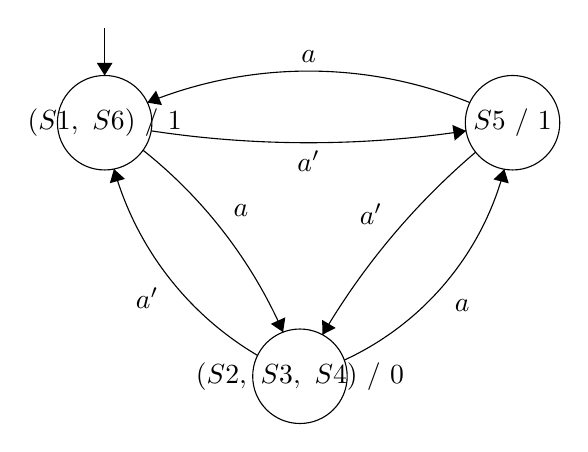
\begin{tikzpicture}[scale=0.2]
            \tikzstyle{every node}+=[inner sep=0pt]
            \draw [black] (36.6,-38.9) circle (3);
            \draw (36.6,-38.9) node {$(S2,\mbox{ }S3,\mbox{ }S4)\mbox{ }/\mbox{ }0$};
            \draw [black] (24.2,-22.8) circle (3);
            \draw (24.2,-22.8) node {$(S1,\mbox{ }S6)\mbox{ }/\mbox{ }1$};
            \draw [black] (50.1,-22.8) circle (3);
            \draw (50.1,-22.8) node {$S5\mbox{ }/\mbox{ }1$};
            \draw [black] (26.912,-21.52) arc (112.10934:67.89066:27.203);
            \fill [black] (26.91,-21.52) -- (27.84,-21.68) -- (27.46,-20.76);
            \draw (37.15,-19.02) node [above] {$a$};
            \draw [black] (47.145,-23.317) arc (-81.36827:-98.63173:66.597);
            \fill [black] (47.15,-23.32) -- (46.28,-22.94) -- (46.43,-23.93);
            \draw (37.15,-24.57) node [below] {$a'$};
            \draw [black] (26.637,-24.547) arc (51.532:23.67395:30.282);
            \fill [black] (35.53,-36.1) -- (35.67,-35.16) -- (34.75,-35.57);
            \draw (32.36,-28.37) node [right] {$a$};
            \draw [black] (33.911,-37.577) arc (-120.49464:-164.29941:20.029);
            \fill [black] (24.79,-25.74) -- (24.53,-26.64) -- (25.49,-26.37);
            \draw (27.64,-33.95) node [left] {$a'$};
            \draw [black] (49.58,-25.751) arc (-14.6444:-65.31589:18.484);
            \fill [black] (49.58,-25.75) -- (48.89,-26.4) -- (49.86,-26.65);
            \draw (46.41,-34.39) node [right] {$a$};
            \draw [black] (38.032,-36.265) arc (149.59133:130.44838:45.501);
            \fill [black] (38.03,-36.26) -- (38.87,-35.83) -- (38.01,-35.32);
            \draw (41.86,-28.62) node [left] {$a'$};
            \draw [black] (24.2,-16.8) -- (24.2,-19.8);
            \fill [black] (24.2,-19.8) -- (24.7,-19) -- (23.7,-19);
            \end{tikzpicture}
        \end{center}
        \hwline
    \end{enumerate}
\end{homeworkProblem}
\pagebreak

%%%%%%%%%%%%%%%%%%%%%%%%%%%%%%%%%%%%%%%%%%%%%%%%%%%%%%%%%%%%%%%%%%%%%%%%%%%%%%%%%%%%%%%%%

\end{document}